\documentclass[11pt]{article}
\usepackage{fullpage,amsmath,amsfonts,mathpazo,microtype,nicefrac,graphicx,verbatimbox,hyperref,listings,enumitem,amssymb,float,fancyhdr}
\hypersetup{
  colorlinks = true,
  allcolors = {cyan}
}

% Margins
% \topmargin=-0.45in
% \evensidemargin=0in
% \oddsidemargin=0in
% \textwidth=6.5in
% \textheight=9.0in
% \headsep=0.25in

% \linespread{1.1} % Line spacing

% % Set up the header and footer
% \pagestyle{fancy}
% \lhead{\hmwkAuthorName} % Top left header
% \chead{\hmwkClass\ (\hmwkClassInstructor\ \hmwkClassTime): \hmwkTitle} % Top center header
% \rhead{\firstxmark} % Top right header
% \lfoot{\lastxmark} % Bottom left footer
% \cfoot{} % Bottom center footer
% \rfoot{Page\ \thepage\ of\ \pageref{LastPage}} % Bottom right footer
% \renewcommand\headrulewidth{0.4pt} % Size of the header rule
% \renewcommand\footrulewidth{0.4pt} % Size of the footer rule

% \setlength\parindent{0pt} % Removes all indentation from paragraphs

%----------------------------------------------------------------------------------------
%   TITLE PAGE
%----------------------------------------------------------------------------------------

\title{
\vspace{1cm}
\textmd{\textbf{AC209a Milestone 5: Data Science with User Ratings and Reviews}}\\
% \normalsize\vspace{0.1in}\small{Due\ on\ \hmwkDueDate}\\
% \vspace{0.1in}\large{\textit{\hmwkClassInstructor\ \hmwkClassTime}}
}

\author{\textbf{Andrew Ross, Sophie Hilgard, Reiko Nishihara, Nick Hoernle}}
\date{\today} % Insert date here if you want it to appear below your name

%----------------------------------------------------------------------------------------

\begin{document}

\maketitle

\section*{Proposal of Future Work}

\paragraph{} In Milestone 4, we evaluated the performance of a number of baseline recommendation models (simple averaging, matrix factorization, popularity ranking, and PageRank) on restaurants and bars in the Yelp dataset. Going forward, and following some of the techniques used in \cite{koren}, we want to see if we can surpass those benchmarks by blending models, computing time-sensitive user and business baseline ratings, and by exploring other models like collaborative filtering. We're also interested in exploring models that exploit more subtle time and location-based effects, as well as continuing to explore the data itself.

\subsection*{Blending}

\paragraph{} One important feature of the Netflix Grand Prize solution, and an increasingly talked about technique in general, is blending predictions from different models to achieve a lower overall error. Concretely, this usually means taking a linear combination of the individual model predictions, where the weights are computed per-example using another model (gradient-boosted decision trees are a popular option \cite{koren,jahrer}). It is also common to train separate blend weight models for different subsets of users \cite{jahrer}, and we've also seen in homeworks that there are also majority vote or selection-based methods for combining predictions, which may be more appropriate for classification tasks (depending on whether you treat predicting ratings as classification or regression -- both perspectives seem to have merit). We plan to explore at least a few of these methods.

\subsection*{Time-sensitive baselines}

\paragraph{} Another important feature of \cite{koren} is the use of time-changing baseline predictors, as well as a frequency baseline that accounts for the number of ratings a user makes in a day, which was important in the Netflix dataset. As we saw in our data exploration, it is also important in the Yelp dataset; 1- and 5-star reviews mean something different coming from a user rating many businesses per day than they do from a user rating just one. We will attempt to evaluate how including each particular term in our the baseline predictors affects our RMSE.

\subsection*{Even more time-sensitive baselines}

\paragraph{} In many ways, time is much more of a factor for Yelpers seeking food or drinks than it is for Netflix users picking their next show. Although public opinion about a show or movie sometimes changes over time, the actual quality of a restaurant's food can change much more rapidly. This can make past restaurant rating data less reliable for predicting future ratings. We're interested in seeing if we can reduce RMSE by weighting recent ratings more heavily when computing baselines, or perhaps trying to detect anomalies. To evaluate performance, however, we may have to test our performance only against recent ratings in our test set.

\paragraph{} Another factor we noticed was that time of day and day of week had a strong correlation with ratings for certain types of businesses. This was especially true for bars and "Nightlife" businesses (shown below), and location also came into play. The plot below shows the ratings that are above the mean in red and the ratings that are below the mean in blue. The average number of ratings per day of the week is shown in the right side vertical axis and the number of ratings on any one day of the year is shown in the axis above the plot. We clearly see that the reviews that are given on Sundays and Mondays tends to be more positive than the reviews given on the other days of the week.

%(shown in figure \ref{fg:bars_nightlife}) 

%\begin{figure}[H]
%\centering
%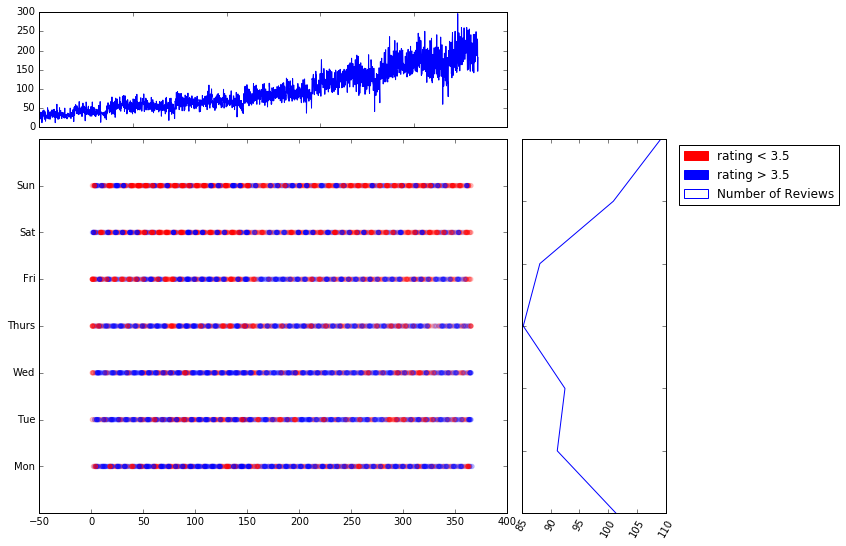
\includegraphics[keepaspectratio=true,scale=0.4]{./images/bars_nightlife_popularity}
%\caption{Plot ratings above and below the mean for days of the week vs days in a year for resturants of categories bar and nightlife in Phoenix}\label{fg:bars_nightlife}
%\end{figure}

%A similar analysis can be applied to various sub locations within the greater Phoenix area. Figure \ref{fg:locations} shows the locations of businesses that are tagged to three cities within the Phoenix area. We can compare the reviews that these locations are receiving over time, as shown in Figures \ref{fg:chandler}, \ref{fg:glendale} and \ref{fg:tempe}.
%\begin{figure}[H]
%\centering
%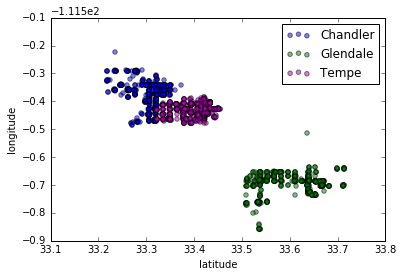
\includegraphics[keepaspectratio=true,scale=0.4]{./images/sub_location_plot}
%\caption{Plot of location of reviews tagged to three cities in Phoenix}\label{fg:locations}
%\end{figure}

%For these different locations we see that to a greater or lesser extent, Sunday reviews receive the highest scores. We also see (focusing on the right hand line plot) that Chandler and Tempe receive roughly 5 and 10 reviews per day more than Glendale. The plot also uses the opacity of the dot to indicate numbers of reviews and there appears to be a trend that in the winter months (days of the year 200 through to 50), the Glendale area is particularly quiet (especially when comparing this to the other cities). Finally, we notice that Glendale appears to be a satellite city within Phoenix could be a possible reason for this.
%\begin{figure}[H]
%\centering
%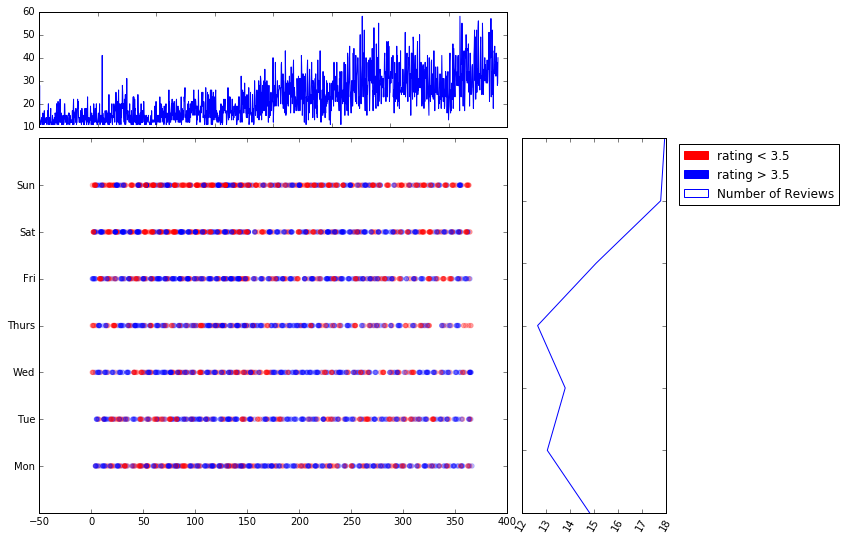
\includegraphics[keepaspectratio=true,scale=0.4]{./images/chandler_restaurants}
%\caption{Plot of reviews above and below the mean for Restaurants in Chandler}\label{fg:chandler}
%\end{figure}

%\begin{figure}[H]
%\centering
%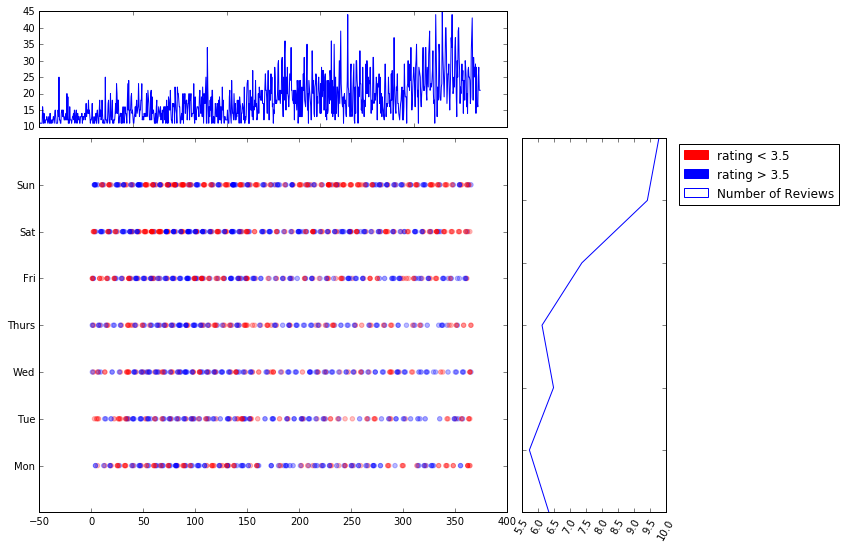
\includegraphics[keepaspectratio=true,scale=0.4]{./images/glendale_restaurants}
%\caption{Plot of reviews above and below the mean for Restaurants in Glendale}\label{fg:glendale}
%\end{figure}

%\begin{figure}[H]
%\centering
%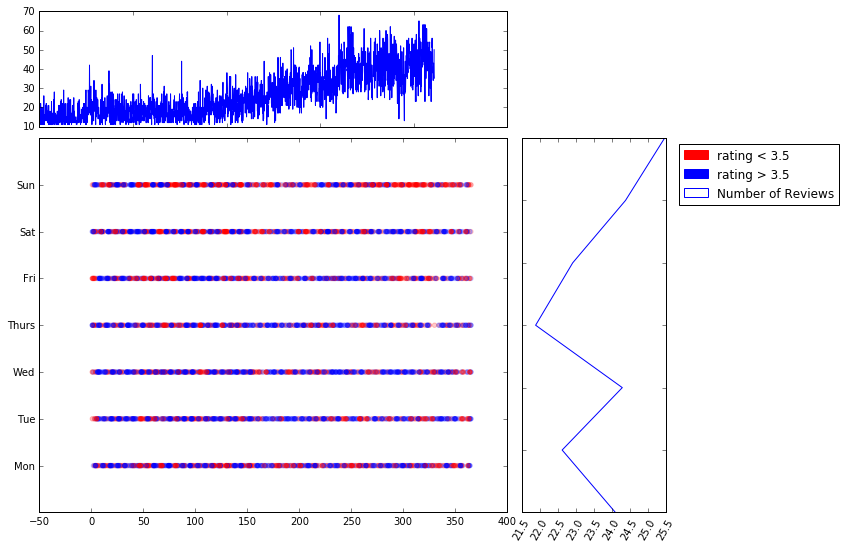
\includegraphics[keepaspectratio=true,scale=0.4]{./images/tempe_restaurants}
%\caption{Plot of reviews above and below the mean for Restaurants in Tempe}\label{fg:tempe}
%\end{figure}

\paragraph{} Weekly or seasonal effects were not something discussed at all in \cite{koren}, perhaps because they aren't as meaningful for movies (It's a Wonderful Life and Bad Santa aside), but we're interested in seeing if we can use them to improve our predictions for restaurants and bars a bit further.

\subsection*{Location-based analysis and going beyond rating RMSE}

\paragraph{} We have also explored a number of other models for predicting business success rather than focusing only on recommendation systems. For example, we can use the Yelp dataset to measure business popularity (using review counts or checkin volume as well as average rating), or even whether and when a business eventually closes. We've spent time investigating location-based, seasonal, and other temporal trends in these business metrics. Location based models have focused largely on clustering methods, as neighborhood is a better predictor than absolute latitude and longitude values. Trend analysis will use regression models over time to analyze if businesses are cyclically popular at any given lag or to find points in time when a given business was comparatively `hot` within its lifetime.

\paragraph{} We also built a network-based recommendation system based roughly on the PageRank algorithm. This model finds the most `connected` business, where path lengths between businesses are weighted inversely to how much a user liked both of the restaurants. To find the next recommendation for any given user, we search the graph built off of similar users and return the `closest` business the user has not yet been to.

\begin{thebibliography}{9}
\bibitem{koren}
  Yehuda Koren,
  \href{http://netflixprize.com/assets/GrandPrize2009_BPC_BellKor.pdf}{The BellKor Solution to the Netflix Grand Prize}
\bibitem{jahrer}
  Michael Jahrer, Andreas Töscher, and Robert Legenstein,
  \href{http://www.igi.tugraz.at/psfiles/JahrerETAL_2010.pdf}{Combining Predictions for an accurate Recommender System}

\end{thebibliography}

\end{document}
